\documentclass[12pt]{article}

\usepackage{sbc-template}

\usepackage{graphicx,url}
\usepackage{amsmath}
\usepackage{algorithm}
\usepackage[noend]{algpseudocode}


\usepackage[brazil]{babel}   
\usepackage[utf8]{inputenc}  

     
\sloppy

\title{Implementação de um Controlador para Redes Definidas por Software com Suporte à Mobilidade}

\author{Iulisloi Zacarias, Luciano Paschoal Gaspary}


\address{Instituto de Informática -- Universidade Federal do Rio Grande do Sul
  (UFRGS)\\
  Caixa Postal 15.064 -- 91.501-970 -- Porto Alegre -- RS -- Brazil
}

\begin{document} 

\maketitle

\begin{abstract}
  This meta-paper describes the style to be used in articles and short papers
  for SBC conferences. For papers in English, you should add just an abstract
  while for the papers in Portuguese, we also ask for an abstract in
  Portuguese (``resumo''). In both cases, abstracts should not have more than
  10 lines and must be in the first page of the paper.
\end{abstract}
     
\begin{resumo} 
  Este meta-artigo descreve o estilo a ser usado na confecção de artigos e
  resumos de artigos para publicação nos anais das conferências organizadas
  pela SBC. É solicitada a escrita de resumo e abstract apenas para os artigos
  escritos em português. Artigos em inglês deverão apresentar apenas abstract.
  Nos dois casos, o autor deve tomar cuidado para que o resumo (e o abstract)
  não ultrapassem 10 linhas cada, sendo que ambos devem estar na primeira
  página do artigo.
\end{resumo}


\section{Introdução}

O consumo e geração de vídeo já é responsável pela maior parte do 
tráfego de dados da internet. Devido à popularização de 
dispositivos móveis como \emph{smartphones} e \emph{tablets}, a 
parcela de tráfego consumida em vídeo tende a crescer ainda mais. 
Este crescimento está relacionado aos serviços oferecidos 
atualmente. Portais de conteúdo gerado pelo usuário (\emph{User 
Generated Content - UGC}) como YouTube e de conteúdo exclusivo 
como o Netflix já são responsáveis pela maior parte dos 
dados consumidos nas redes que compõem a internet nos Estados 
Unidos~\cite{narayanan2014} e contabilizam aproximadamente 67\% dos 
dados trafegados na rede mundial. Projeções baseadas em 
estudos~\cite{cisco2016} apontam um crescimento estimado em 30\% no 
consumo de vídeo pela internet até 2020.

As conexões utilizadas por \emph{streaming} de vídeo em geral são 
de longa duração e, durante este espaço de tempo, apresentam 
requisitos rígidos de latência, variação de latência e vazão de 
dados pela rede. Para a entrega de uma boa experiência ao usuário 
que está assistindo ao vídeo, a rede precisa suportar estes 
requisitos~\cite{narayanan2014}. Em um ambiente heterogêneo e que 
muitas vezes apresenta mobilidade, tanto do nó consumidor como em 
alguns casos dos nós que estão gerando o fluxo de vídeo, manter estes requisitos dos serviços em patamares aceitáveis é um grande desafio dada a alta complexidade de gerenciar os equipamentos que compõem a rede (\emph{switches} e roteadores). Esta complexidade que emerge acaba dificultando e restringindo o desenvolvimento de soluções mais criativas e otimizadas para cenários com características mais específicas, como as já citadas aplicações de vídeo.

Redes definidas por software (SDN) são uma tecnologia emergente e constituem um novo paradigma na área de transmissão de dados. Possuem características que permitem grande inovação, tornando possível simplificar e centralizar o gerenciamento dos equipamentos. Em contraste às atuais redes IPs, que apesar da grande utilização e disseminação nos mais variados ambientes, são complexos e difíceis de gerenciar~\cite{Kreutz2015}. A aplicação de políticas mais complexas nas redes convencionais normalmente requer que os operadores acessem cada um dos equipamentos a serem configurados e realizem estas operações utilizando um conjunto de funções específicas e que mudam de fabricante para fabricante.

Além das características citadas acima, estas redes apresentam alta dinamicidade e capacidade de adaptação, ótimo \emph{custo x benefício} tornando elas ideais para ambientes instáveis ou ambientes que apresentam mudanças constantes, como cenários de mobilidade \emph{wireless}. A proposta desta nova arquitetura de redes é separá-la em duas camadas, uma camadas superior de controle e uma camada inferior chamada de camada de dados ou camada de encaminhamento de pacotes~\cite{Jammal2014}.

Este trabalho apresenta o protótipo de um controlador para redes definidas por software com suporte à movimentação dos clientes entre os \emph{switches} da rede, capaz de encontrar o menor caminho que os pacotes de dados devem seguir deste o cliente até um servidor de \emph{stream}. Quando os \emph{hosts} da rede se movem, o controlador é capaz de reconhecer esta movimentação e de acordo com a nova topologia estabelecer um melhor caminho para encaminhamento dos pacotes de dados.

\section{Trabalhos Relacionados}

\section{Descrição do cenário e solução implementada}
Esta seção têm por objetivo descrever o cenário utilizado no desenvolvimento do controlador, particularidades do experimento e ferramentas e tecnologias utilizadas.

\subsection{Cenário}
A topologia da rede modelada no Mininet para o desenvolvimento e testes é representada na Figura~\ref{fig:topology}. Esta topologia consiste de dez equipamentos do tipo \emph{switch} e oito equipamentos do tipo \emph{access point}. Apesar da diferenciação entre os tipos de equipamentos na figura, na simulação realizada no software Mininet todos os equipamentos são do tipo \emph{switch} e se comportam de forma semelhante, isso porque a versão do software utilizada não disponibiliza componentes com suporte à redes sem fio.

\begin{figure}[ht]
\centering
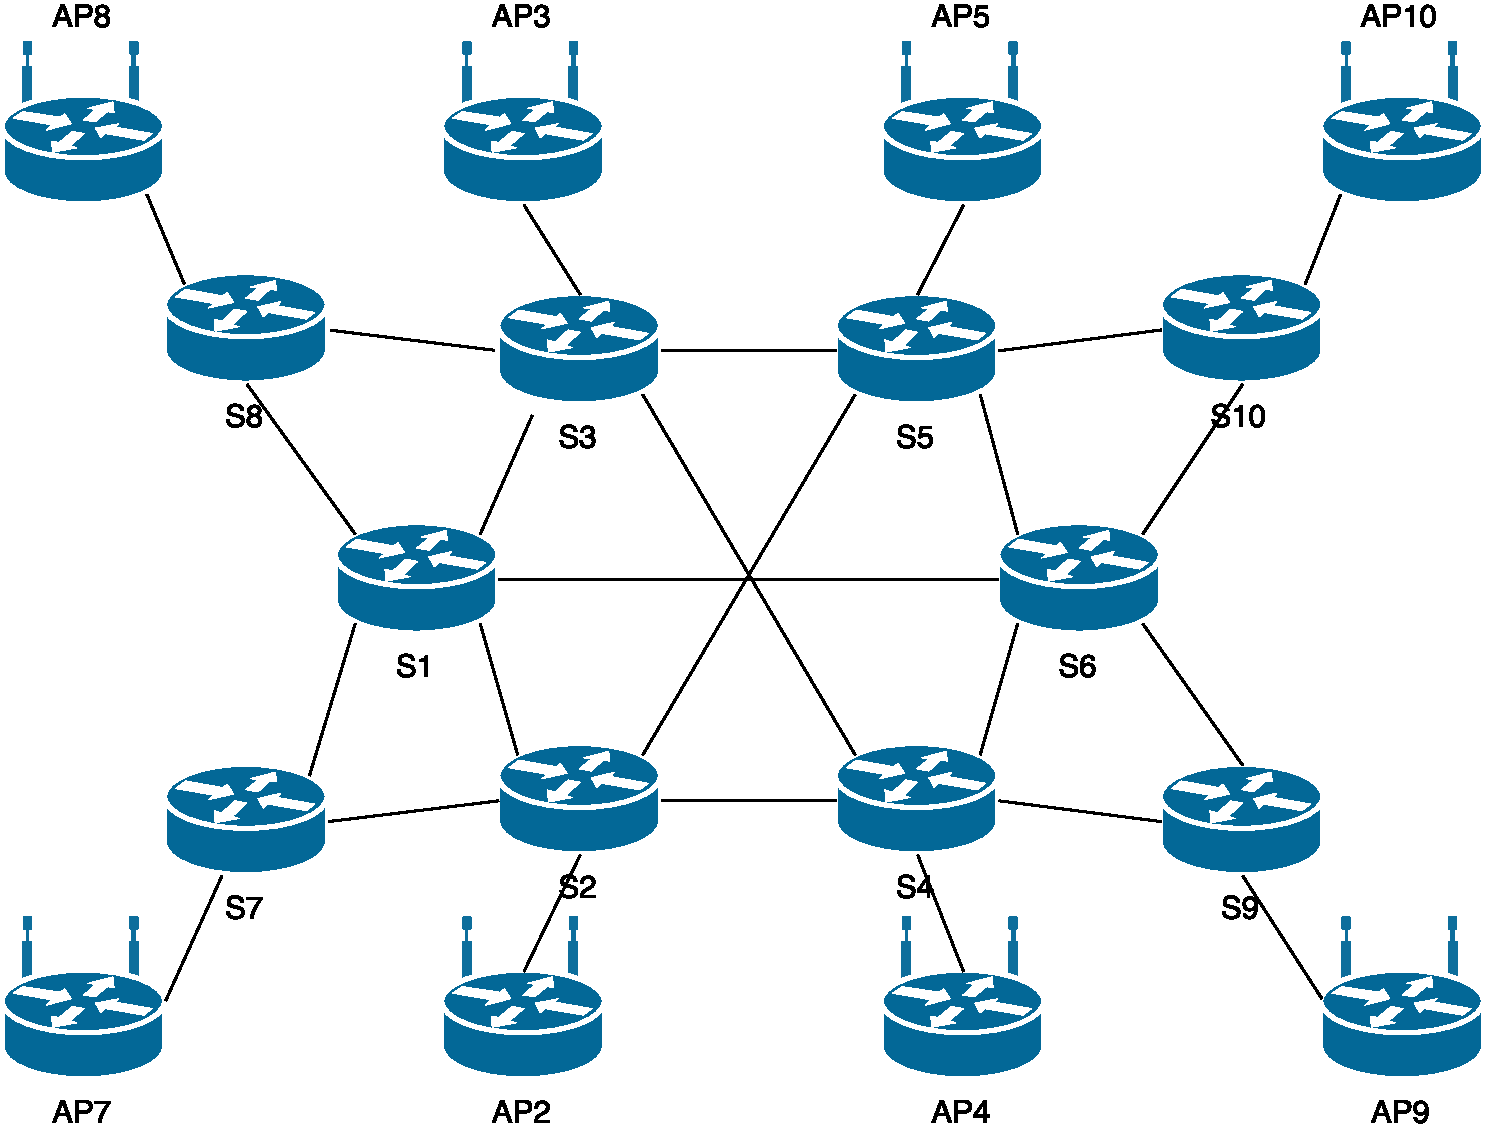
\includegraphics[width=.60\textwidth]{figures/scenario.pdf}
\caption{Topologia de rede empregada no desenvolvimento e teste do controlador. Os clientes podem se conectar em qualquer \emph{switch} ou \emph{acess point}.}
\label{fig:topology}
\end{figure}

O cenário utilizado no processo de teste e avaliação, considera apenas um \emph{host} com a função de servidor de vídeo, enquanto o número de clientes pode variar de um até oito clientes. O servidor é responsável por disponibilizar um fluxo de vídeo que será consumido pelos \emph{hosts} clientes. Os \emph{hosts} clientes consomem o fluxo de vídeo, utilizando um \emph{player} de vídeo e geram estatísticas e registros de \emph{log} dos eventos percebidos por eles. Os \emph{links} que interligam os elementos \emph{switch} da rede e estes aos \emph{hosts} possuem capacidade virtual de 10.000~Mbps, estabelecida por padrão pelo software simulador.

Todos os componentes da rede simulada são compatíveis com o protocolo para redes definidas por software OpenFlow versão 1.3. Os \emph{switches} utilizados na simulação utilizam o software de controle Open vSwitch versão 2.0.2.

\subsection{Ferramentas utilizadas no ambiente}
O ambiente de utilizado neste trabalho durante o desenvolvimento e testes foi criado e simulado utilizando a ferramenta Mininet. O software Mininet é 

\subsection{Algoritmo utilizado}



\section{Conclusões e trabalhos futuros}

\section{First Page} \label{sec:firstpage}

The first page must display the paper title, the name and address of the
authors, the abstract in English and ``resumo'' in Portuguese (``resumos'' are
required only for papers written in Portuguese). The title must be centered
over the whole page, in 16 point boldface font and with 12 points of space
before itself. Author names must be centered in 12 point font, bold, all of
them disposed in the same line, separated by commas and with 12 points of
space after the title. Addresses must be centered in 12 point font, also with
12 points of space after the authors' names. E-mail addresses should be
written using font Courier New, 10 point nominal size, with 6 points of space
before and 6 points of space after.

The abstract and ``resumo'' (if is the case) must be in 12 point Times font,
indented 0.8cm on both sides. The word \textbf{Abstract} and \textbf{Resumo},
should be written in boldface and must precede the text.

\section{CD-ROMs and Printed Proceedings}

In some conferences, the papers are published on CD-ROM while only the
abstract is published in the printed Proceedings. In this case, authors are
invited to prepare two final versions of the paper. One, complete, to be
published on the CD and the other, containing only the first page, with
abstract and ``resumo'' (for papers in Portuguese).

\section{Sections and Paragraphs}

Section titles must be in boldface, 13pt, flush left. There should be an extra
12 pt of space before each title. Section numbering is optional. The first
paragraph of each section should not be indented, while the first lines of
subsequent paragraphs should be indented by 1.27 cm.

\subsection{Subsections}

The subsection titles must be in boldface, 12pt, flush left.

\section{Figures and Captions}\label{sec:figs}


Figure and table captions should be centered if less than one line
(Figure~\ref{fig:exampleFig1}), otherwise justified and indented by 0.8cm on
both margins, as shown in Figure~\ref{fig:exampleFig2}. The caption font must
be Helvetica, 10 point, boldface, with 6 points of space before and after each
caption.

\begin{figure}[ht]
\centering
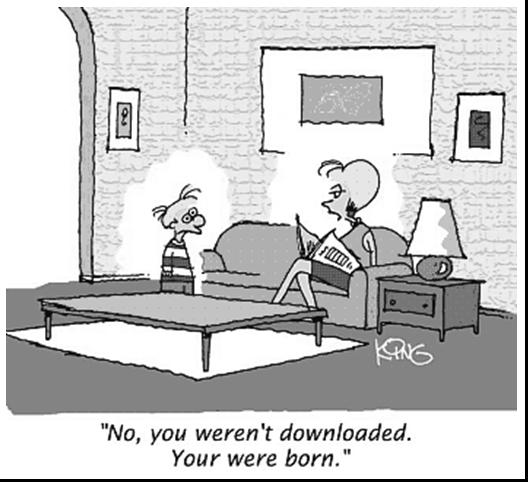
\includegraphics[width=.5\textwidth]{fig1.jpg}
\caption{A typical figure}
\label{fig:exampleFig1}
\end{figure}

\begin{figure}[ht]
\centering
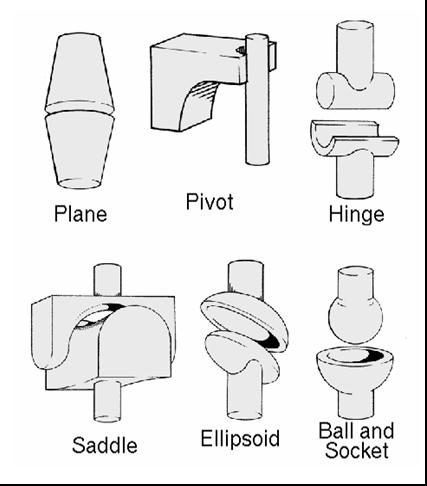
\includegraphics[width=.3\textwidth]{fig2.jpg}
\caption{This figure is an example of a figure caption taking more than one
  line and justified considering margins mentioned in Section~\ref{sec:figs}.}
\label{fig:exampleFig2}
\end{figure}

In tables, try to avoid the use of colored or shaded backgrounds, and avoid
thick, doubled, or unnecessary framing lines. When reporting empirical data,
do not use more decimal digits than warranted by their precision and
reproducibility. Table caption must be placed before the table (see Table 1)
and the font used must also be Helvetica, 10 point, boldface, with 6 points of
space before and after each caption.

\begin{table}[ht]
\centering
\caption{Variables to be considered on the evaluation of interaction
  techniques}
\label{tab:exTable1}
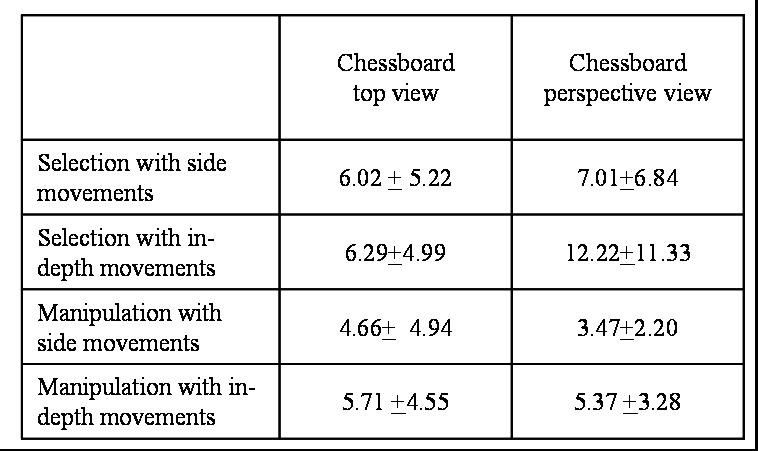
\includegraphics[width=.7\textwidth]{table.jpg}
\end{table}

\section{Images}

All images and illustrations should be in black-and-white, or gray tones,
excepting for the papers that will be electronically available (on CD-ROMs,
internet, etc.). The image resolution on paper should be about 600 dpi for
black-and-white images, and 150-300 dpi for grayscale images.  Do not include
images with excessive resolution, as they may take hours to print, without any
visible difference in the result. 

\section{References}

Bibliographic references must be unambiguous and uniform.  We recommend giving
the author names references in brackets, e.g. \cite{knuth:84},
\cite{boulic:91}, and \cite{smith:99}.

The references must be listed using 12 point font size, with 6 points of space
before each reference. The first line of each reference should not be
indented, while the subsequent should be indented by 0.5 cm.

\bibliographystyle{sbc}
\bibliography{sbc-template}

\end{document}
